\documentclass{beamer}
\usepackage{listings}
\usepackage{xcolor}

% Define the dark theme colors
\definecolor{background}{RGB}{30,30,30}
\definecolor{foreground}{RGB}{220,220,220}
\definecolor{keyword}{RGB}{255,120,50}
\definecolor{string}{RGB}{50,200,50}
\definecolor{comment}{RGB}{150,150,150}

% Set up the Scala language listings
\lstdefinelanguage{Scala}{
  keywords={abstract, as, case, catch, class, def, do, enum, else, erased, extends, extension, false, final, finally, for, given, if, implicit, into, import, lazy, match, new, null, object, override, package, private, protected, return, sealed, super, this, throw, tracked, trait, try, true, type, using, val, var, while, with, yield},
  morekeywords={=>,<-,<\%,>:,\#,@},
  sensitive=true,
  comment=[l]{//},
  morecomment=[s]{/*}{*/},
  string=[b]",
  morestring=[b]',
  morestring=[b]"""
}

\lstset{
  language=Scala,
  backgroundcolor=\color{background},
  basicstyle=\ttfamily\color{foreground}\footnotesize,
  keywordstyle=\color{keyword}\bfseries,
  stringstyle=\color{string},
  commentstyle=\color{comment}\itshape,
  numberstyle=\tiny\color{foreground},
  numbersep=5pt,
  tabsize=2,
  showspaces=false,
  showstringspaces=false,
  breaklines=true,
  frame=single,
  rulecolor=\color{foreground},
  frameround=ffff,
  captionpos=b
}

\mode<presentation> {
  \usetheme{Madrid} % Change this to any other theme if needed
  \setbeamercolor{normal text}{bg=background, fg=foreground}
  \setbeamercolor{section in toc}{fg=foreground}
}

\AtBeginSection[]{
  \begin{frame}
  \vfill
  \centering
  \begin{beamercolorbox}[sep=8pt,center,shadow=true,rounded=true]{title}
    \usebeamerfont{title}\insertsectionhead\par%
  \end{beamercolorbox}
  \vfill
  \end{frame}
}

\title[Scala 3 features you haven't used (yet)]{Scala 3 features \\
you probably haven’t used \\
(yet)}
\author{Kacper Korban (VirtusLab)}
\date{\today}

\begin{document}

\begin{frame}
  \titlepage%
\end{frame}

\begin{frame}
  \frametitle{Why?}

  \centering
  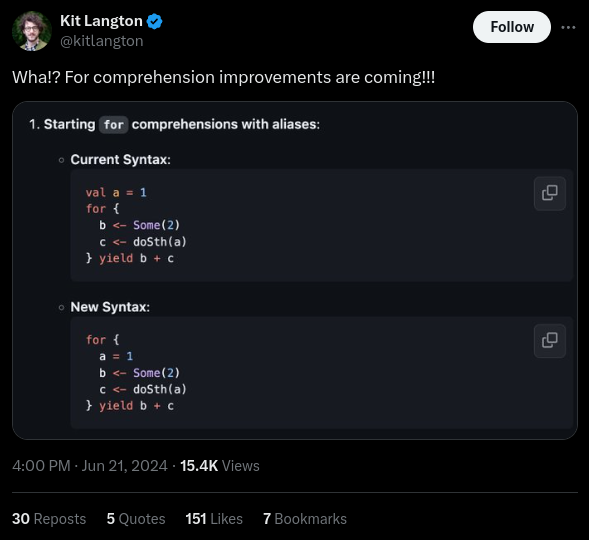
\includegraphics[width=0.7\textwidth]{kitx.png}
  
\end{frame}

\begin{frame}
  \frametitle{What is this talk about?}

  \begin{itemize}
    \item Overview of experimental Scala 3 features
    \item Motivation for adding them
    \item Overview of some incoming experimental features
    \item Plus a bonus
  \end{itemize}

\end{frame}

\begin{frame}
  \frametitle{A solution to survive boring parts: A Jumping Frog}

  \begin{itemize}
    \item You are standing in front of a pond.
    \item There is a path with some final number stone tiles going to the middle of the pond in a single line.
    \item There's also an invisible frog that is standing on a random stone tile.
    \item After each unit of time the frog jumps forward or backwards by exactly one tile. The frog cannot exit the path.
    \item Your task is to catch the frog, by standing on the same tile as the frog at some point in time.
    \item You can move by at most one tile in any direction on the path.
    \item You always move at the same time as the frog.
  \end{itemize}

  \textbf{
  Come up with an algorithm that will ensure you can catch the frog and prove its correctness.
  }

\end{frame}

% \begin{frame}
%   \frametitle{Outline}
%   \tableofcontents
% \end{frame}

\begin{frame}
  \frametitle{About Me}

  \begin{itemize}
    \item Scala Developer at VirtusLab (formerly at Scala 3 team)
    \item GitHub/X: @KacperFKorban
  \end{itemize}

  \vspace{1cm}

  \begin{columns}[T]
    \begin{column}{.5\textwidth}
      OSS projects I have meaningful contributions to:
      \begin{itemize}
        \item scala/scala3 (compiler + scaladoc)
        \item softwaremill/quicklens
        \item softwaremill/magnolia
        \item VirtusLab/besom
      \end{itemize}
    \end{column}

    \begin{column}{.5\textwidth}
      OSS Projects I created:
      \begin{itemize}
        \item VirtusLab/Inkuire --- Hoogle for Scala
        \item VirtusLab/avocADO --- parallel for-comprehensions
        \item KacperFKorban/GUInep --- automatic UI forms for functions
      \end{itemize}
    \end{column}
  \end{columns}
\end{frame}

\section{Experimental Features}

\begin{frame}[fragile]
  \frametitle{namedTypeArguments}
  \begin{itemize}
    \item \textbf{Feature Name:} namedTypeArguments
    \item \textbf{Import:} \texttt{import scala.language.experimental.namedTypeArguments}
    \item \textbf{TLDR:} Allows you to specify type arguments of functions by name.
  \end{itemize}
\end{frame}

\begin{frame}[fragile]
  \frametitle{namedTypeArguments --- Example}

  This language feature allows us to write the following code:
  \begin{lstlisting}
  def foo[A, B, C](a: A, b: B, c: C): Unit = ???

  foo[A = Int, B = String, C = Boolean](1, "2", true)
  \end{lstlisting}

  An obvious benefit is improved readability.

\end{frame}

\begin{frame}[fragile]
  \frametitle{namedTypeArguments --- Motivation}

  Consider the following code with a potential inference error:

  \begin{lstlisting}
  def foo[A, B, C, D, E](a: A, b: B, c: C, d: D, e: E): Unit = ???

  foo(a1, b1, c1, d1, e1) // error can't infer type C
  \end{lstlisting}

  \pause\

  To fix this, we would need to instantiate all type parameters:

  \begin{lstlisting}
  foo[A1, B1, C1, D1, E1](a1, b1, c1, d1, e1)
  \end{lstlisting}

  \pause\

  With named type arguments, we can write:

  \begin{lstlisting}
  foo[C = C1](a1, b1, c1, d1, e1)
  \end{lstlisting}
  
\end{frame}

\begin{frame}[fragile]
  \frametitle{genericNumberLiterals}
  \begin{itemize}
    \item \textbf{Feature Name:} genericNumberLiterals
    \item \textbf{Import:} \texttt{import scala.language.experimental.genericNumberLiterals}
    \item \textbf{TLDR:} Allows for using number literals for custom number types.
  \end{itemize}
\end{frame}

\begin{frame}[fragile]
  \frametitle{genericNumberLiterals --- Usage}

  With this language feature, we can define a custom number type like this:

  \begin{lstlisting}
  case class MyInt(value: Int):
    override def toString = value.toString()
  
  object MyInt:
    def apply(digits: String): MyInt =
      MyInt(digits.toInt)
    given FromDigits[MyInt] with
      def fromDigits(digits: String) = MyInt(digits)

  val myInt: MyInt = 123
  \end{lstlisting}
  
\end{frame}

\begin{frame}[fragile]
  \frametitle{genericNumberLiterals --- Usage}

  There are 4 alternative typeclasses we can define:

  \begin{lstlisting}
  // for parsing integers (e.g. 123)
  FromDigits[T]
  // for parsing decimal numbers (e.g. 123.45)
  FromDigits.Decimal[T]
  // for parsing integers with a radix (e.g. 0x123)
  FromDigits.WithRadix[T]
  // for parsing floating numbers with exponent
  // (e.g. 1.23e-4)
  FromDigits.Floating[T]
  \end{lstlisting}

\end{frame}

\begin{frame}[fragile]
  \frametitle{erasedDefinitions}
  \begin{itemize}
    \item \textbf{Feature Name:} erasedDefinitions
    \item \textbf{Import:} \texttt{import scala.language.experimental.erasedDefinitions}
    \item \textbf{TLDR:} Allows for defining erased definitions.
  \end{itemize}
\end{frame}

\begin{frame}[fragile]
  \frametitle{erasedDefinitions --- Motivation}

  Let's consider the following code:

  \begin{lstlisting}
    sealed trait State
    final class On extends State
    final class Off extends State
    
    class IsOff[S <: State]
    object IsOff:
      given isOff: IsOff[Off] = new IsOff[Off]
    
    class Machine[S <: State]:
      def turnedOn(using IsOff[S]): Machine[On] = new Machine[On]
    
    val m = new Machine[Off]
    m.turnedOn.turnedOn // error
  \end{lstlisting}

  The \texttt{IsOff[T]} parameter isn't used in runtime.
  
\end{frame}

\begin{frame}[fragile]
  \frametitle{erasedDefinitions --- Motivation}

  We can add the \texttt{erased} keyword to the \texttt{IsOff} implicit parameter:

  \begin{lstlisting}
    sealed trait State
    final class On extends State
    final class Off extends State
    
    class IsOff[S <: State]
    given isOff: IsOff[Off] = new IsOff[Off]
    
    class Machine[S <: State]:
      def turnedOn(using erased IsOff[S]): Machine[On] = new Machine[On]
      // def turnedOn(): Machine = new Machine()
    
    val m = new Machine[Off]
    m.turnedOn.turnedOn // error
  \end{lstlisting}

  \small
  This way, the \texttt{IsOff[T]} parameter is not present in the generated bytecode.

  The compiler also checks that \texttt{erased} parameters aren't used in computations.
  
\end{frame}

\begin{frame}[fragile]
  \frametitle{erasedDefinitions --- Motivation}

  We can also mark classes as \texttt{erased}. The following will achieve the same effect: 

  \begin{lstlisting}
    sealed trait State
    final class On extends State
    final class Off extends State
    
    erased class IsOff[S <: State]
    given isOff: IsOff[Off] = new IsOff[Off]
    
    class Machine[S <: State]:
      def turnedOn(using IsOff[S]): Machine[On] = new Machine[On]
      // def turnedOn(): Machine = new Machine()
    
    val m = new Machine[Off]
    m.turnedOn.turnedOn // error
  \end{lstlisting}

  All usages of \texttt{erased} classes are marked as \texttt{erased}.
  
\end{frame}

\begin{frame}[fragile]
  \frametitle{clauseInterleaving}
  \begin{itemize}
    \item \textbf{Feature Name:} clauseInterleaving
    \item \textbf{Import:} \texttt{import scala.language.experimental.clauseInterleaving}
    \item \textbf{TLDR:} Allows for interleaving type parameter clauses and term clauses.
  \end{itemize}
\end{frame}

\begin{frame}[fragile]
  \frametitle{clauseInterleaving --- Motivation}

  Let's consider the following code that defines a key-value store:

  \begin{lstlisting}
  trait Key:
    type Value
  
  class Store:
    def getOrElse(key: Key)(default: => key.Value): key.Value = ...
  \end{lstlisting}

  We would also like to allow for the default value to be passed a supertype of \texttt{key.Value}.

  Like in e.g. \texttt{Option}.

  \begin{lstlisting}
  trait Option[+A]:
    final def getOrElse[B >: A](default: => B): B
  \end{lstlisting}
  
\end{frame}

\begin{frame}[fragile]
  \frametitle{clauseInterleaving --- Motivation}

  We might want to attempt to write the following code that contains a forward reference:

  \begin{lstlisting}
  class Store:
    def getOrElse[V >: key.Value](key: Key)(default: => V): V = ...
  \end{lstlisting}

  \pause\

  Clause interleaving allows us to write the following code:

  \begin{lstlisting}
  class Store:
    def getOrElse(key: Key)[V >: key.Value](default: => V): V = ...
  \end{lstlisting}

\end{frame}

\begin{frame}
  \frametitle{clauseInterleaving --- Restrictions}

  There are some restrictions to clause interleaving:

  \begin{itemize}
    \item No type currying --- the following is not allowed: \lstinline{def foo[T][U](t: T, u: U): Unit}
    \item No clause interleaving in class definitions. (but \texttt{apply} methods are OK)
    \item No clause interleaving in lhs of extension methods.
  \end{itemize}

\end{frame}

% \begin{frame}[fragile]
%   \frametitle{pureFunctions + captureChecking}
%   \begin{itemize}
%     \item \textbf{Feature Name:} pureFunctions + captureChecking
%     \item \textbf{Import:} \texttt{import scala.language.experimental.pureFunctions} \\ \texttt{import scala.language.experimental.captureChecking}
%     \item \textbf{TLDR:} Allows defining pure functions (with ->) and enables tracking of captured variables.
%   \end{itemize}
% \end{frame}

% \begin{frame}[fragile]
%   \frametitle{pureFunctions + captureChecking --- Motivation}

%   Let's consider this infamous example:

%   \begin{lstlisting}
%   def usingLogFile[T](op: FileOutputStream => T): T =
%     val logFile = FileOutputStream("log")
%     val result = op(logFile)
%     logFile.close()
%     result
  
%   val later = usingLogFile { file => () => file.write(0) }
%   later() // crash stream closed
%   \end{lstlisting}
  
% \end{frame}

% \begin{frame}[fragile]
%   \frametitle{pureFunctions + captureChecking --- Motivation}

%   We can track the lifetime of \texttt{FileOutputStream}:

%   \begin{lstlisting}
%   def usingLogFile[T](op: FileOutputStream^ => T): T =
%     val logFile = FileOutputStream("log")
%     val result = op(logFile)
%     logFile.close()
%     result
  
%   val later = usingLogFile { file => () => file.write(0) }
%   later() // compile error
%   \end{lstlisting}

%   \pause\

%   pureFunctions allows us to define function types that do not capture variables:

%   \begin{lstlisting}
%   def mapPure[A, B](f: A -> B): List[A] -> List[B] = ...
%   \end{lstlisting}

% \end{frame}

\section{Bigger experimental features}

\begin{frame}[fragile]
  \frametitle{into --- Background (implicitConversions)}

  Ols style implicit conversions (\texttt{implicit def}) give feature warnings in Scala 3 on declaration. 
  There are plans to deprecate them in the far future.

  \begin{lstlisting}
  case class Msg(msg: String)

  implicit def stringToMsg(i: String): Msg = Msg(i) // feature warning
  \end{lstlisting}

  We should enable implicit conversions explicitly:

  \begin{lstlisting}
  import scala.language.implicitConversions
  \end{lstlisting}
\end{frame}

\begin{frame}[fragile]
  \frametitle{into --- Background (implicitConversions)}

  New style implicit conversions give feature warnings in Scala 3 on use.

  \begin{lstlisting}
  case class Msg1(msg: String)

  given Conversion[String, Msg1] with
    def apply(i: String): Msg1 = Msg1(i)

  val str = "hello"
  val msg1: Msg1 = str // feature warning
  println(msg1)
  \end{lstlisting}

  We should again enable implicit conversions explicitly again:

  \begin{lstlisting}
  import scala.language.implicitConversions
  \end{lstlisting}
\end{frame}

\begin{frame}[fragile]
  \frametitle{into}
  \begin{itemize}
    \item \textbf{Feature Name:} into
    \item \textbf{Import:} \texttt{import scala.language.experimental.into}
    \item \textbf{TLDR:} Allows implicit conversions to be used on a specified parameter.
  \end{itemize}
\end{frame}

\begin{frame}[fragile]
  \frametitle{into --- Motivation}

  The following code shows a common pattern in Scala:

  \begin{lstlisting}
  enum MyList[+A]:
    case MyNil
    case MyCons(head: A, tail: MyList[A])

    def toList: List[A] = this match
      case MyNil => Nil
      case MyCons(h, t) => h +: t.toList

  given [A]: Conversion[MyList[A], List[A]] =
    (x: MyList[A]) => x.toList

  def loopOver[A](it: List[A])(f: A => Unit): Unit =
    it.iterator.foreach(f)

  val myLst = MyList.MyCons(1, MyList.MyNil)
  loopOver(myLst)(x => println(x)) // feature warning
  \end{lstlisting}

\end{frame}

\begin{frame}[fragile]
  \frametitle{into --- Motivation}

  \texttt{into} allows us to write the following code, that will not give a feature warning at use site.

  \begin{lstlisting}
  enum MyList[+A]:
    case MyNil
    case MyCons(head: A, tail: MyList[A])

  def toList: List[A] = this match
    case MyNil => Nil
    case MyCons(h, t) => h +: t.toList

  given [A]: Conversion[MyList[A], List[A]] =
    (x: MyList[A]) => x.toList

  def loopOver[A](it: into List[A])(f: A => Unit): Unit =
    it.iterator.foreach(f)

  val myLst = MyList.MyCons(1, MyList.MyNil)
  loopOver(myLst)(x => println(x))
  \end{lstlisting}

  Note: \texttt{into} on varargs allows conversions on all varargs arguments.

\end{frame}

\begin{frame}[fragile]
  \frametitle{namedTuples}
  \begin{itemize}
    \item \textbf{Feature Name:} namedTuples
    \item \textbf{Import:} \texttt{import scala.language.experimental.namedTuples}
    \item \textbf{TLDR:} Allows you to name tuples.
  \end{itemize}
\end{frame}

\begin{frame}[fragile]
  \frametitle{namedTuples --- Motivation}

  Consider the following code:

  \begin{lstlisting}
  def analyzeString(input: String): (Int, Int) = {
    val it = input.iterator
    var l = 0
    var count = 0
    while (it.hasNext) {
      val c = it.next()
      l += 1
      if ("AEIOUaeiou".contains(c)) count += 1
    }
    (l, count)
  }
  \end{lstlisting}
  
\end{frame}

\begin{frame}[fragile]
  \frametitle{namedTuples --- Motivation}

  We can rewrite the code using named tuples, to make the code more readable:

  \begin{lstlisting}
  def analyzeString(
    input: String
  ): (length: Int, vowelsCount: Int) = {
    val it = input.iterator
    var l = 0
    var count = 0
    while (it.hasNext) {
      val c = it.next()
      l += 1
      if ("AEIOUaeiou".contains(c)) count += 1
    }
    (length = l, vowelsCount = count)
  }
  \end{lstlisting}

\end{frame}

\begin{frame}[fragile]
  \frametitle{namedTuples --- Motivation}

  Another good use case is database operations (specifically results of joins):

  \begin{lstlisting}
  def joinTables(
    t1: Table1,
    t2: Table2
  ): List[(id: Int, name: String, age: Int, address: String)] =
    for
      ...
    yield
      (
        id = person.id,
        name = person.name,
        age = person.age,
        address = address.address
      )
  \end{lstlisting}

  Slightly different library that might benefit from this is: VirtusLab/iskra

\end{frame}

\begin{frame}[fragile]
  \frametitle{namedTuples --- Motivation}

  Somewhat unrelated addition of this feature: named pattern matching not only for classes.

  \begin{lstlisting}
  case class City(name: String, population: Int)

  def getCityInfo(city: City) =
    city match
      case c @ City(name = "Paris") =>
        "Paris is the capital of France"
      case City(population = 0) =>
        "This city is uninhabited"
      case City(name = n, population = p) =>
        s"$n has $p inhabitants"    
  \end{lstlisting}

\end{frame}

\begin{frame}[fragile]
  \frametitle{modularity}
  \begin{itemize}
    \item \textbf{Feature Name:} modularity
    \item \textbf{Import:} \texttt{import scala.language.experimental.modularity}
    \item \textbf{TLDR:} Allows for dependent class parameters and new type class style.
  \end{itemize}
\end{frame}

\begin{frame}[fragile]
  \frametitle{modularity --- Motivation}

  Consider the following code:

  \begin{lstlisting}
  class C:
    type T

  def f(x: C): x.T = ...

  val y: C { type T = Int }

  val _: Int = f(y)
  \end{lstlisting}

  \begin{lstlisting}
  class F(val x: C):
    val result: x.T = ...
  
  val _: Int = F(y).result // type error
  \end{lstlisting}

  Currently Scala is dependently typed for functions but not for classes.

\end{frame}

\begin{frame}[fragile]
  \frametitle{modularity --- Motivation}

  Consider the following OCaml style type class module definition:

  \begin{lstlisting}
  trait Ordering:
    type T
    def compare(t1:T, t2: T): Int
  
  class OrderedSet(val ord: Ordering):
    type Set = List[ord.T]
  
    def empty: Set = Nil
    extension (s: Set)
      def add(x: ord.T): Set = ...

  object intOrdering extends Ordering:
    type T = Int
    def compare(t1: T, t2: T): Int = t1 - t2
  
  val IntSet = new OrderedSet(intOrdering)

  val set = IntSet.empty.add(6).add(8).add(23) // type error
  \end{lstlisting}
  
\end{frame}

\begin{frame}[fragile]
  \frametitle{modularity --- Motivation}

  We can fix the code by making the \texttt{ord} parameter tracked:

  \begin{lstlisting}
  trait Ordering:
    type T
    def compare(t1:T, t2: T): Int
  
  class OrderedSet(tracked val ord: Ordering):
    type Set = List[ord.T]
  
    def empty: Set = Nil
    extension (s: Set)
      def add(x: ord.T): Set = ...

  object intOrdering extends Ordering:
    type T = Int
    def compare(t1: T, t2: T): Int = t1 - t2
  
  val IntSet = new OrderedSet(intOrdering)

  val set = IntSet.empty.add(6).add(8).add(23)
  \end{lstlisting}

\end{frame}

\begin{frame}[fragile]
  \frametitle{modularity --- Underlying intuition}

  The intuition behind tracked class parameters is thinking of the constructor as returning the declared class with a refinement to the class paremeter.

  e.g.

  \begin{lstlisting}
  class OrderedSet(tracked val ord: Ordering) // : OrderedSet { val ord: ord.type }
  \end{lstlisting}

\end{frame}

\begin{frame}[fragile]
  \frametitle{modularity type class improvements --- Motivation}

  Currently we define type classes like this:

  \begin{lstlisting}
  trait ShowOld[T]:
    extension (x: T) def show: String
  
  trait SemiGroupOld[T]:
    extension (x: T) def combine(y: T): T
  
  trait MonoidOld[T] extends SemiGroupOld[T]:
    def unit: T
  \end{lstlisting}

\end{frame}

\begin{frame}[fragile]
  \frametitle{modularity type class improvements --- Motivation}

  We create instances of type classes and use them like this:

  \begin{lstlisting}
  given ShowOld[Int] with
    extension (x: Int) def show = x.toString
  
  given [T: ShowOld] => ShowOld[List[T]] with
    extension (xs: List[T]) def show = xs.map(_.show).mkString("[", ", ", "]")
  
  def combineAllOld[T: MonoidOld](xs: List[T]): T =
    // requires summon
    xs.foldLeft(summon[MonoidOld].unit)(_.combine(_))

  def combineAllOld1[T](
    xs: List[T]
  )(using m: MonoidOld[T]): T = // explicit using
    xs.foldLeft(m.unit)(_.combine(_))
  \end{lstlisting}

\end{frame}

\begin{frame}[fragile]
  \frametitle{modularity type class improvements --- Motivation}

  The new modularity feature allows us to define type classes like this:

  \begin{lstlisting}
  trait Show:
    type Self // Self is the type, we are defining the type class for
    extension (x: Self) def show: String

  trait SemiGroup:
    type Self
    extension (x: Self) def combine(y: Self): Self

  trait Monoid extends SemiGroup:
    def unit: Self
  \end{lstlisting}

\end{frame}

\begin{frame}[fragile]
  \frametitle{modularity type class improvements --- Motivation}

  We define instances and use them like this:

  \begin{lstlisting}
  given Int is Show: // `Int is Show` is equivalent for Show { type Self = Int }
    extension (x: Int) def show = x.toString

  given [T: Show] => List[T] is Show:
    extension (xs: List[T]) def show = xs.map(_.show).mkString("[", ", ", "]")

  def combineAll[T: Monoid as m](xs: List[T]): T = // `as` creates an alias
    xs.foldLeft(m.unit)(_.combine(_))

  def combineAll1[T: Monoid](xs: List[T]): T = // default alias `T`
    xs.foldLeft(T.unit)(_.combine(_))
  \end{lstlisting}

\end{frame}

\begin{frame}[fragile]
  \frametitle{modularity type class improvements --- Motivation}

  We also have new syntax for aggregate type class instances:

  \begin{lstlisting}
  def combineAllAndPrint[T: {Monoid, Show}](xs: List[T]): T =
    xs.foldLeft(T.unit)(_.combine(_)).tap(x => println(T.show(x)))

  def combineAllAndPrint1[T: {Monoid as m, Show as s}](xs: List[T]): T =
    xs.foldLeft(m.unit)(_.combine(_)).tap(x => println(s.show(x)))
  \end{lstlisting}

\end{frame}

\section{Bonus}

\begin{frame}[fragile]
  \frametitle{Bonus --- setters in Scala}

  Let's consider the rules for defining field setters in Scala:

  \begin{lstlisting}
  class ClassWithAGetterAndASetter:
    private var _value: Int = 0
    def value: Int = _value
    def value_=(newValue: Int): Unit = _value = newValue

  val c = ClassWithAGetterAndASetter()

  println(c.value)

  c.value = 2 // c.value_=(2)

  println(c.value) // 2
  \end{lstlisting}

\end{frame}

\begin{frame}[fragile]
  \frametitle{Bonus --- unary operators in Scala}

  Next, let's take a look at the rules for defining unary operators in Scala:

  \begin{lstlisting}
  class ClassWithUnaryOp:
    private var i: Int = 1
    def unary_! : Int = -i

  val cwo = ClassWithUnaryOp()

  println(!cwo) // -1
  \end{lstlisting}

\end{frame}


\begin{frame}[fragile]
  \frametitle{Bonus --- putting it together}

  Can we combine them together?

  \begin{lstlisting}
  class AClass(private var i: Int):
    def unary_! : Int = i
    def unary_!_=(i: Int): Unit = this.i = i // parsing error
  \end{lstlisting}

\end{frame}

\begin{frame}[fragile]
  \frametitle{Bonus --- putting it together}

  What if we use backticks?

  \begin{lstlisting}
  class AClass(private var i: Int):
    def unary_! : Int = i
    def `unary_!_=`(i: Int): Unit = this.i = i
  
  val ac = AClass(1)

  println(!ac)

  !ac = 2 // ac.`unary_!_=`(2)

  println(!ac)
  \end{lstlisting}

  Works!

\end{frame}

\section{Incoming experimental features}

\begin{frame}[fragile]
  \frametitle{betterFors}
  \begin{itemize}
    \item \textbf{Feature Name:} betterFors
    \item \textbf{Import:} \texttt{import scala.language.experimental.betterFors}
    \item \textbf{TLDR:} Simplifies desugaring of for-comprehensions and allows them to start with an alias.
  \end{itemize}
\end{frame}

\begin{frame}[fragile]
  \frametitle{betterFors --- Motivation}

  Currently, we are often forced to write code like this:

  \begin{lstlisting}
  val a = 1
  for {
    b <- Some(2)
    c <- doSth(a)
  } yield b + c
  \end{lstlisting}

  \pause\

  With the new changes, we will be able to write:

  \begin{lstlisting}
  for {
    a = 1
    b <- Some(2)
    c <- doSth(a)
  } yield b + c
  \end{lstlisting}
  
\end{frame}

\begin{frame}[fragile]
  \frametitle{betterFors --- Motivation}
  
  Let's consider the following code:

  \begin{lstlisting}
  for {
    a <- doSth(arg)
    b = a
  } yield a + b
  \end{lstlisting}

  Currently desugars to:

  \begin{lstlisting}
  doSth(arg).map { a =>
    val b = a
    (a, b)
  }.map { case (a, b) => a + b }
  \end{lstlisting}

  \pause\

  New desugaring:

  \begin{lstlisting}
  doSth(arg).map { a =>
    val b = a
    a + b
  }
  \end{lstlisting}

\end{frame}

\begin{frame}[fragile]
  \frametitle{betterFors --- Motivation}
  
  Let's consider the following code:

  \begin{lstlisting}
  for {
    a <- List(1, 2, 3)
  } yield a
  \end{lstlisting}

  Currently desugars to:

  \begin{lstlisting}
  List(1, 2, 3).map(a => a)
  \end{lstlisting}

  \pause\

  New desugaring:

  \begin{lstlisting}
  List(1, 2, 3)
  \end{lstlisting}

\end{frame}

\begin{frame}[fragile]
  \frametitle{alternativeBindPatterns}
  \begin{itemize}
    \item \textbf{Feature Name:} alternativeBindPatterns
    \item \textbf{Import:} \texttt{-}
    \item \textbf{TLDR:} Allows binds in alternative pattern matches.
  \end{itemize}
\end{frame}

\begin{frame}[fragile]
  \frametitle{alternativeBindPatterns --- Motivation}

  Consider the following code:

  \begin{lstlisting}
  enum Command:
    case Get, North, Go, Pick, Up
    case Item(name: String)
  
  import Command.*
  \end{lstlisting}

  \pause\

  We might want write the following code:

  \begin{lstlisting}
  def loop(cmds: List[Command]): Unit =
    cmds match
      case Pick :: Up :: Item(name) :: Nil =>
        ???
      case Get :: Item(name) :: Nil =>
        ???
  \end{lstlisting}
\end{frame}

\begin{frame}[fragile]
  \frametitle{alternativeBindPatterns --- Motivation}

  The following code will be more expressive:

  \begin{lstlisting}
  def loop(cmds: List[Command]): Unit =
    cmds match
      case Pick :: Up :: Item(name) :: Nil |
           Get :: Item(name) :: Nil =>
        ???
  \end{lstlisting}

\end{frame}

\begin{frame}[fragile]
  \frametitle{multipleAssignments}
  \begin{itemize}
    \item \textbf{Feature Name:} multipleAssignments
    \item \textbf{Import:} \texttt{-}
    \item \textbf{TLDR:} Allows multiple assignments in a single statement.
  \end{itemize}
\end{frame}

\begin{frame}[fragile]
  \frametitle{multipleAssignments --- Motivation}

  The following code implements a Fibonacci sequence iterator:

  \begin{lstlisting}
  class FibonacciIterator() extends Iterator[Int]:
    private var a: Int = 0
    private var b: Int = 1
  
    def hasNext = true
    def next() =
      val r = a
      val n = a + b
      a = b
      b = n
      r
  \end{lstlisting}

  The semantics aren't clear, because of the temporary variable \texttt{n}.
\end{frame}

\begin{frame}[fragile]
  \frametitle{multipleAssignments --- Motivation}

  With the new proposal, it can be rewritten as:

  \begin{lstlisting}
  class FibonacciIterator() extends Iterator[Int]:
    private var a: Int = 0
    private var b: Int = 1
  
    def hasNext = true
    def next() =
      val r = a
      (a, b) = (b, a + b)
      r
  \end{lstlisting}
  
  \pause\

  Acceptance criteria:
  \begin{itemize}
    \item single level tuple on the left
    \item any expression that returns a tuple of the correct type on the right
  \end{itemize}

  % Acceptane criteria:
  % - single level tuple on the left
  % - any expression that returns a tuple of the correct type on the right
\end{frame}

\begin{frame}
  \frametitle{Thank you!}
  \begin{center}
    \Huge
    Questions?
  \end{center}
\end{frame}

\end{document}
